%% ==================== Problem 1 ====================
\subsection{Problem 1}

\textbf{Question:} Show that the loglinear random effects model
\[
  \log[E(Y_{it}\mid \boldsymbol{b}_i)] = \boldsymbol{x}_{it}'\boldsymbol{\beta} + \boldsymbol{z}_{it}'\boldsymbol{b}_i,
\]
where $\{\boldsymbol{b}_i\}$ are independent $N(\boldsymbol{0}, \boldsymbol{\Sigma})$, implies the marginal loglinear model
\[
  \log[E(Y_{it})] = \boldsymbol{x}_{it}'\boldsymbol{\beta} + \frac{1}{2}\boldsymbol{z}_{it}'\boldsymbol{\Sigma}\boldsymbol{z}_{it},
\]
with the same fixed effects but with offset term. Explain why $\frac{1}{2}\boldsymbol{z}_{it}'\boldsymbol{\Sigma}\boldsymbol{z}_{it}$ is an offset term.

(Hint: use the moment generating function for a normal variable $\boldsymbol{b} \sim N(\boldsymbol{\mu}, \boldsymbol{\Sigma})$: $E(\exp(\boldsymbol{t}'\boldsymbol{b})) = \exp(\boldsymbol{t}'\boldsymbol{\mu} + \frac{1}{2}\boldsymbol{t}'\boldsymbol{\Sigma}\boldsymbol{t})$)

\bigskip
\textbf{Solution:}

由条件期望的定义：
\[
  E(Y_{it}\mid \boldsymbol{b}_i) = \exp(\boldsymbol{x}_{it}'\boldsymbol{\beta} + \boldsymbol{z}_{it}'\boldsymbol{b}_i).
\]

对随机效应 $\boldsymbol{b}_i$ 取期望，得边际期望：
\begin{align*}
  E(Y_{it}) &= E_{\boldsymbol{b}_i}\big[E(Y_{it}\mid \boldsymbol{b}_i)\big] \\
  &= E_{\boldsymbol{b}_i}\big[\exp(\boldsymbol{x}_{it}'\boldsymbol{\beta} + \boldsymbol{z}_{it}'\boldsymbol{b}_i)\big] \\
  &= \exp(\boldsymbol{x}_{it}'\boldsymbol{\beta}) \cdot E\big[\exp(\boldsymbol{z}_{it}'\boldsymbol{b}_i)\big].
\end{align*}

由于 $\boldsymbol{b}_i \sim N(\boldsymbol{0}, \boldsymbol{\Sigma})$，利用正态分布的矩生成函数（MGF），取 $\boldsymbol{t} = \boldsymbol{z}_{it}$，$\boldsymbol{\mu} = \boldsymbol{0}$：
\[
  E\big[\exp(\boldsymbol{z}_{it}'\boldsymbol{b}_i)\big] = \exp\!\Big(\boldsymbol{0}'\boldsymbol{z}_{it} + \frac{1}{2}\boldsymbol{z}_{it}'\boldsymbol{\Sigma}\boldsymbol{z}_{it}\Big) = \exp\!\Big(\frac{1}{2}\boldsymbol{z}_{it}'\boldsymbol{\Sigma}\boldsymbol{z}_{it}\Big).
\]

因此：
\[
  E(Y_{it}) = \exp(\boldsymbol{x}_{it}'\boldsymbol{\beta}) \cdot \exp\!\Big(\frac{1}{2}\boldsymbol{z}_{it}'\boldsymbol{\Sigma}\boldsymbol{z}_{it}\Big) = \exp\!\Big(\boldsymbol{x}_{it}'\boldsymbol{\beta} + \frac{1}{2}\boldsymbol{z}_{it}'\boldsymbol{\Sigma}\boldsymbol{z}_{it}\Big).
\]

取对数得边际对数线性模型：
\[
  \log[E(Y_{it})] = \boldsymbol{x}_{it}'\boldsymbol{\beta} + \frac{1}{2}\boldsymbol{z}_{it}'\boldsymbol{\Sigma}\boldsymbol{z}_{it}.
\]

\textbf{关于 offset term 的解释：} offset term（偏移项）是在模型中不参与参数估计的已知项，其系数固定为1。此处 $\frac{1}{2}\boldsymbol{z}_{it}'\boldsymbol{\Sigma}\boldsymbol{z}_{it}$ 由已知的协变量 $\boldsymbol{z}_{it}$ 和已知的协方差矩阵 $\boldsymbol{\Sigma}$ 构成，不需要进行估计，因此是 offset term。另外，由于 $\exp$ 变换不是线性的，因此需要进行均值的修正。


%% ==================== Problem 2 ====================
\subsection{Problem 2}

\textbf{Question:} Let $\boldsymbol{Y}_1, \ldots, \boldsymbol{Y}_n$ be independent random vectors, where $\boldsymbol{Y}_i = (Y_{i1}, Y_{i2})^T$ are two repeated measurements from subject $i$. Assume that
\[
  E(Y_{ij}) = \mu_{ij} = \beta_0 + x_i\beta_1, \quad \text{Var}(Y_{ij}) = \sigma^2, \quad i=1,\ldots,n,\; j=1,2
\]
where the subject-level covariates $x_i$ are iid variables and the variance $\sigma^2$ are known. Also assume that $\text{corr}(Y_{i1}, Y_{i2}) = \alpha$, where $\alpha > 0$ is known.

\begin{enumerate}[label=(\alph*)]
  \item Write down the matrices $V_i = \text{Var}(\boldsymbol{Y}_i)$ and
  \[
    D_i = \begin{pmatrix} \frac{\partial \mu_{i1}}{\partial \beta_0} & \frac{\partial \mu_{i1}}{\partial \beta_1} \\[4pt] \frac{\partial \mu_{i2}}{\partial \beta_0} & \frac{\partial \mu_{i2}}{\partial \beta_1} \end{pmatrix}.
  \]
  Calculate the following terms: $D_i^T V_i^{-1} D_i$, $D_i^T D_i$, and $D_i^T V_i D_i$.

  \item Let $\widehat{\boldsymbol{\beta}}_E = (\widehat{\beta}_{0E}, \widehat{\beta}_{1E})$ denote the estimate of $\boldsymbol{\beta}$ under a GEE model with an exchangeable correlation structure, and $\widehat{\boldsymbol{\beta}}_I = (\widehat{\beta}_{0I}, \widehat{\beta}_{1I})$ denote the estimate of $\boldsymbol{\beta}$ under a GEE model with an independent correlation structure. Show their asymptotic variances (avar) to be
  \[
    n\,\text{avar}(\widehat{\boldsymbol{\beta}}_E) = \bigg(\lim_{n\to\infty} \frac{1}{n}\sum_{i=1}^n D_i^T V_i^{-1} D_i\bigg)^{-1}
  \]
  \[
    n\,\text{avar}(\widehat{\boldsymbol{\beta}}_I) = \bigg(\lim_{n\to\infty}\frac{1}{n}\sum_{i=1}^n D_i^T D_i\bigg)^{-1} \bigg(\lim_{n\to\infty}\frac{1}{n}\sum_{i=1}^n D_i^T V_i D_i\bigg) \bigg(\lim_{n\to\infty}\frac{1}{n}\sum_{i=1}^n D_i^T D_i\bigg)^{-1}
  \]

  \item Evaluate the asymptotic relative efficiency of $\widehat{\beta}_{1E}$ (the slope estimator) versus $\widehat{\beta}_{1I}$:
  \[
    \lim_{n\to\infty} \frac{n\,\text{avar}(\widehat{\beta}_{1E})}{n\,\text{avar}(\widehat{\beta}_{1I})}.
  \]
\end{enumerate}

\bigskip
\textbf{Solution:}

\begin{enumerate}[label=(\alph*)]
\item 由题意，$\mu_{ij} = \beta_0 + x_i\beta_1$，因此
\[
  D_i = \begin{pmatrix} 1 & x_i \\ 1 & x_i \end{pmatrix}.
\]

协方差矩阵为
\[
  V_i = \text{Var}(\boldsymbol{Y}_i) = \begin{pmatrix} \sigma^2 & \alpha\sigma^2 \\ \alpha\sigma^2 & \sigma^2 \end{pmatrix} = \sigma^2 \begin{pmatrix} 1 & \alpha \\ \alpha & 1 \end{pmatrix}.
\]

其逆矩阵为
\[
  V_i^{-1} = \frac{1}{(1-\alpha^2)\sigma^2} \begin{pmatrix} 1 & -\alpha \\ -\alpha & 1 \end{pmatrix}.
\]

计算各矩阵乘积：
\[
  D_i^T V_i^{-1} D_i = \frac{1}{(1-\alpha^2)\sigma^2} \begin{pmatrix} 2 & 2x_i \\ 2x_i & 2x_i^2 \end{pmatrix} = \frac{2}{(1-\alpha^2)\sigma^2} \begin{pmatrix} 1 & x_i \\ x_i & x_i^2 \end{pmatrix}.
\]

\[
  D_i^T D_i = \begin{pmatrix} 1 & 1 \\ x_i & x_i \end{pmatrix} \begin{pmatrix} 1 & x_i \\ 1 & x_i \end{pmatrix} = \begin{pmatrix} 2 & 2x_i \\ 2x_i & 2x_i^2 \end{pmatrix} = 2\begin{pmatrix} 1 & x_i \\ x_i & x_i^2 \end{pmatrix}.
\]

\[
  D_i^T V_i D_i = \sigma^2 \begin{pmatrix} 1 & 1 \\ x_i & x_i \end{pmatrix} \begin{pmatrix} 1 & \alpha \\ \alpha & 1 \end{pmatrix} \begin{pmatrix} 1 & x_i \\ 1 & x_i \end{pmatrix} = 2\sigma^2(1+\alpha) \begin{pmatrix} 1 & x_i \\ x_i & x_i^2 \end{pmatrix}.
\]

\item GEE 的估计方程为
\[
  \sum_{i=1}^n D_i^T V_i^{-1}(\boldsymbol{Y}_i - \boldsymbol{\mu}_i) = \boldsymbol{0}.
\]
记 $U_i(\boldsymbol{\beta}) = D_i^T V_i^{-1}(\boldsymbol{Y}_i - \boldsymbol{\mu}_i)$，则
\[
  \frac{\partial U_i}{\partial \boldsymbol{\beta}} = D_i^T V_i^{-1}\Big(-\frac{\partial \boldsymbol{\mu}_i}{\partial \boldsymbol{\beta}}\Big) = -D_i^T V_i^{-1} D_i.
\]

\textbf{对于 $\widehat{\boldsymbol{\beta}}_E$}（exchangeable correlation，即 working correlation matrix 结构正确）：由于工作相关矩阵与真实相关矩阵一致，GEE 是有效的，因此
\[
  \text{avar}(\widehat{\boldsymbol{\beta}}_E) = \left[\lim_{n\to\infty}\sum_{i=1}^n D_i^T V_i^{-1} D_i\right]^{-1}.
\]
即
\[
  n\,\text{avar}(\widehat{\boldsymbol{\beta}}_E) = \left[\lim_{n\to\infty}\frac{1}{n}\sum_{i=1}^n D_i^T V_i^{-1} D_i\right]^{-1}.
\]

\textbf{对于 $\widehat{\boldsymbol{\beta}}_I$}（independent correlation，即 working correlation matrix 结构不正确）：记工作协方差矩阵为 $W_i = \sigma^2 I_2$，则 $W_i^{-1} = \frac{1}{\sigma^2}I_2$。GEE 的稳健方差估计为
\[
  \text{avar}(\widehat{\boldsymbol{\beta}}_I) = A^{-1} B A^{-1},
\]
其中
\[
  A = \lim_{n\to\infty}\sum_{i=1}^n D_i^T W_i^{-1} D_i = \lim_{n\to\infty}\sum_{i=1}^n D_i^T D_i \cdot \frac{1}{\sigma^2},
\]
\[
  B = \lim_{n\to\infty}\sum_{i=1}^n D_i^T W_i^{-1} V_i W_i^{-1} D_i = \lim_{n\to\infty}\sum_{i=1}^n D_i^T V_i D_i \cdot \frac{1}{\sigma^4}.
\]

代入并整理得
\[
  n\,\text{avar}(\widehat{\boldsymbol{\beta}}_I) = \bigg(\lim_{n\to\infty}\frac{1}{n}\sum_{i=1}^n D_i^T D_i\bigg)^{-1} \bigg(\lim_{n\to\infty}\frac{1}{n}\sum_{i=1}^n D_i^T V_i D_i\bigg) \bigg(\lim_{n\to\infty}\frac{1}{n}\sum_{i=1}^n D_i^T D_i\bigg)^{-1}.
\]

\item 将 (a) 和 (b) 的结果代入。记
\[
  M = \begin{pmatrix} 1 & E(x_i) \\ E(x_i) & E(x_i^2) \end{pmatrix}.
\]

则
\[
  \lim_{n\to\infty}\frac{1}{n}\sum_{i=1}^n D_i^T V_i^{-1} D_i = \frac{2}{\sigma^2(1-\alpha)} M, \quad
  \lim_{n\to\infty}\frac{1}{n}\sum_{i=1}^n D_i^T D_i = 2M,
\]
\[
  \lim_{n\to\infty}\frac{1}{n}\sum_{i=1}^n D_i^T V_i D_i = 2\sigma^2(1+\alpha) M.
\]

因此
\[
  n\,\text{avar}(\widehat{\boldsymbol{\beta}}_E) = \frac{\sigma^2(1-\alpha)}{2} M^{-1},
\]
\[
  n\,\text{avar}(\widehat{\boldsymbol{\beta}}_I) = \frac{1}{2}M^{-1} \cdot 2\sigma^2(1+\alpha)M \cdot \frac{1}{2}M^{-1} = \frac{\sigma^2(1+\alpha)}{2} M^{-1}.
\]

对于 $\widehat{\beta}_{1E}$ 和 $\widehat{\beta}_{1I}$，取上述矩阵的 $(2,2)$ 元素即可，因此
\[
  \lim_{n\to\infty} \frac{n\,\text{avar}(\widehat{\beta}_{1E})}{n\,\text{avar}(\widehat{\beta}_{1I})} = \frac{1-\alpha}{1+\alpha}.
\]
\end{enumerate}


%% ==================== Problem 3 ====================
\subsection{Problem 3}

\textbf{Question:} Consider the subject-specific model for binary matched pairs.
\begin{enumerate}[label=(\alph*)]
  \item Using the conditional likelihood, show the closed form of the MLE $\widehat{\beta}$.
  \item Derive the SE estimator for the MLE, which is based on the Fisher information matrix $I_n(\beta)$.
  \item Show that the score test for testing $\beta = 0$ is equivalent to McNemar's test. Note that the score statistic has the form $U(0)^2/I_n(0)$, where $U(0)$ and $I_n(0)$ are the score function and Fisher information matrix evaluated at $\beta = 0$.
  \item The binary matched pair data can be organized in $n$ $2\times 2$ contingency tables. We know that the Mantel-Haenszel estimator of a common odds ratio in the $n\times 2\times 2$ is
  \[
    \widehat{\theta}_{MH} = \frac{\sum_{k=1}^n n_{k11}n_{k22}/n_{k\cdot\cdot}}{\sum_{k=1}^n n_{k12}n_{k21}/n_{k\cdot\cdot}}.
  \]
  Show that $\widehat{\theta}_{MH}$ simplifies to $\exp(\widehat{\beta})$ for the $n\times 2\times 2$ tables for binary matched pair data.
\end{enumerate}

\bigskip
\textbf{Solution:}

符号定义与课程讲义相同。设 binary matched pair 数据中，$(Y_{i1}, Y_{i2})$ 的四种可能结果对应频数为 $n_{11}$（1,1）、$n_{22}$（0,0）、$n_{12}$（1,0）、$n_{21}$（0,1）。

\begin{enumerate}[label=(\alph*)]
\item 条件似然函数（conditioning on the marginal totals）为
\[
  CL(\beta) = \frac{\exp(\beta\, n_{12})}{[1+\exp(\beta)]^{n_{12}+n_{21}}}.
\]

对 $\beta$ 求导并令其为零：
\[
  \frac{\partial CL(\beta)}{\partial \beta} = \frac{n_{12}\exp(\beta\, n_{12})[1+\exp(\beta)]^{n_{12}+n_{21}} - \exp(\beta\, n_{12})(n_{12}+n_{21})[1+\exp(\beta)]^{n_{12}+n_{21}-1}\exp(\beta)}{[1+\exp(\beta)]^{2(n_{12}+n_{21})}} = 0.
\]

化简得
\[
  n_{12}(1+\exp(\beta)) - (n_{12}+n_{21})\exp(\beta) = 0 \implies n_{12} - n_{21}\exp(\beta) = 0.
\]

因此
\[
  \widehat{\beta} = \log\!\left(\frac{n_{12}}{n_{21}}\right).
\]

验证 $\frac{\partial^2 CL(\beta)}{\partial \beta^2} < 0$ 及边界条件即得上式为 MLE。

\item 对数条件似然为
\[
  \ell(\beta) = \log CL(\beta) = \beta\, n_{12} - (n_{12}+n_{21})\log(1+\exp(\beta)).
\]

Score function：
\[
  U(\beta) = \frac{\partial \ell(\beta)}{\partial \beta} = n_{12} - (n_{12}+n_{21})\frac{\exp(\beta)}{1+\exp(\beta)}.
\]

二阶导数：
\[
  \frac{\partial^2 \ell(\beta)}{\partial \beta^2} = -(n_{12}+n_{21})\left[\frac{\exp(\beta)}{1+\exp(\beta)} - \frac{(\exp(\beta))^2}{(1+\exp(\beta))^2}\right] = -(n_{12}+n_{21})\frac{\exp(\beta)}{(1+\exp(\beta))^2}.
\]

Fisher information：
\[
  I(\beta) = -E\!\left[\frac{\partial^2 \ell(\beta)}{\partial \beta^2}\right] = (n_{12}+n_{21})\frac{\exp(\beta)}{(1+\exp(\beta))^2}.
\]

代入 $\widehat{\beta} = \log\frac{n_{12}}{n_{21}}$，得
\[
  \text{SE}(\widehat{\beta}) = \left(\frac{1}{I(\widehat{\beta})}\right)^{1/2} = \left(\frac{n_{12}+n_{21}}{n_{12}\,n_{21}}\right)^{1/2}.
\]

\item Score statistic 为 $U(0)^2 / I_n(0)$。

其中
\[
  I_n(0) = \frac{n_{12}+n_{21}}{4},
\]
\[
  U(0) = n_{12} - (n_{12}+n_{21})\cdot\frac{1}{2} = \frac{1}{2}(n_{12}-n_{21}).
\]

代入得
\[
  \frac{U(0)^2}{I_n(0)} = \frac{\frac{1}{4}(n_{12}-n_{21})^2}{\frac{n_{12}+n_{21}}{4}} = \frac{(n_{12}-n_{21})^2}{n_{12}+n_{21}},
\]
与 McNemar 检验统计量一致。

\item 由 (a) 知 $\exp(\widehat{\beta}) = n_{12}/n_{21}$。

对于 binary matched pair 数据的 $n\times 2\times 2$ 表格，考虑第 $k$ 个配对：

\begin{center}
\begin{tabular}{c|cc|c}
\toprule
配对类型 & $n_{k11}$ & $n_{k12}$ & 分子贡献 \\
\midrule
(1,1): $n_{k11}$ & $\begin{smallmatrix}1 & 0\\1 & 0\end{smallmatrix}$ & & 0 \\
(0,0): $n_{k22}$ & $\begin{smallmatrix}0 & 1\\0 & 1\end{smallmatrix}$ & & 0 \\
(1,0): $n_{k12}$ & $\begin{smallmatrix}1 & 0\\0 & 1\end{smallmatrix}$ & & $\frac{1}{2}$ \\
(0,1): $n_{k21}$ & $\begin{smallmatrix}0 & 1\\1 & 0\end{smallmatrix}$ & & 0 \\
\bottomrule
\end{tabular}
\end{center}

类似地，分母中只有 (0,1) 类型有贡献 $\frac{1}{2}$。因此
\[
  \widehat{\theta}_{MH} = \frac{\frac{1}{2}n_{12}}{\frac{1}{2}n_{21}} = \frac{n_{12}}{n_{21}} = \exp(\widehat{\beta}).
\]
\end{enumerate}


%% ==================== Problem 4 ====================
\subsection{Problem 4}

\textbf{Question:} (Framingham Data) We are interested in studying the relationship between an individual's BMI (as a time-varying variable) and his/her cholesterol levels, using the longitudinal data of all three exams. The cholesterol levels can be taken either as a continuous variable (log-transformed) or a binary variable indicating ``undesirable'' versus ``desirable'' (as defined previously) using the ``desirable'' as the reference. In addressing this question, your model should properly capture the pattern of change in cholesterol levels over time (the ``PERIOD'' variable), and it is also important to adjust for age group (as a categorical variable) and sex. Both the population-average effect and the individual-specific effects of BMI on cholesterol status are of interest. Specifically, you should follow these steps:

\begin{enumerate}[label=(\alph*)]
  \item Plot the individual trajectories of the (log-transformed) continuous cholesterol level. What is the pattern of change in cholesterol levels over time, linear or quadratic? Model your observed pattern in the following models.
  \item Fit a LMM for the (log-transformed) continuous cholesterol level. Hint: include covariates BMI, period, age group, and sex.
  \item Fit a GLMM for the binary cholesterol status.
  \item Fit a GEE for the binary cholesterol status.
  \item Compare your results for the relationship between BMI and cholesterol statuses from GLMM and GEE. Explain the difference.
\end{enumerate}

\bigskip
\textbf{Solution:}

我们使用 Framingham data，探讨 BMI 与胆固醇水平之间的关系。由于受试者在多个时期进行重复测量且受试者具有异质性，因此观测值之间存在相关性，使用普通的回归方法分析没有利用到这方面的信息。

我们分别将胆固醇水平视为：连续变量（log-cholesterol）、二分类变量（undesirable vs desirable cholesterol status），分别建立 LMM、GLMM、GEE 模型，以研究 BMI 对胆固醇水平的影响，同时考虑时间、年龄组及性别等协变量。

\begin{enumerate}[label=(\alph*)]
\item 由于样本量较大，若直接绘制所有个体的 trajectory，会导致图像过于密集十分难以辨认。因此我们随机抽取了 100 名受试者进行绘图（见图）。

\begin{center}
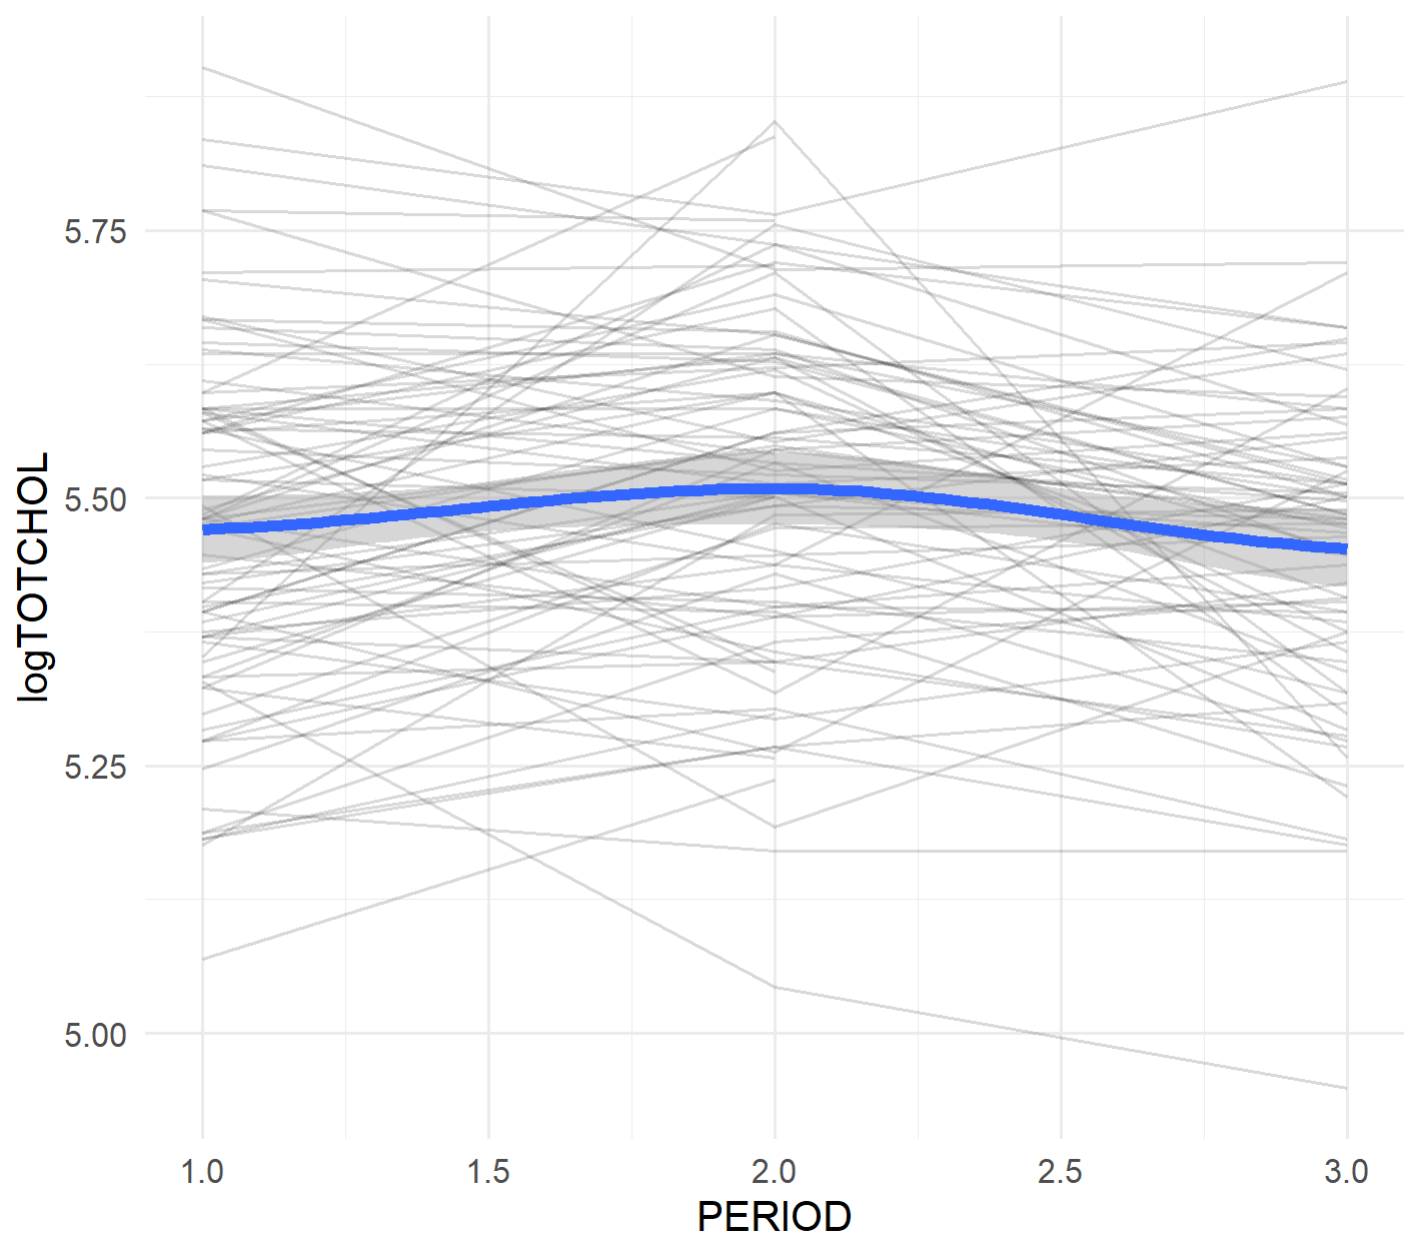
\includegraphics[width=0.8\textwidth]{figs/hw7_trajectory_plot.png}
\end{center}

从图中可以看出，胆固醇水平（取对数）随时间大致稳定，呈现先轻微上升后轻微下降的规律，视觉上并不十分明显，因此进一步进行分析。为了减少线性项和二次项之间的共线性，对 PERIOD 进行中心化处理 \texttt{period\_c=PERIOD-2}，随后比较 linear model 和 quadratic model，结果显示 likelihood ratio test 的 ANOVA $p < 2.2\times 10^{-16}$，即便考虑模型复杂度的惩罚，采用 BIC 进行分析，结果亦有二次模型 BIC 数值更低。

\begin{center}
\begin{tabular}{lcc}
\toprule
 & df & BIC \\
\midrule
linear model & 8 & $-10129$ \\
quadratic model & 9 & $-10738$ \\
\bottomrule
\end{tabular}
\end{center}

以上说明引入二次项可以显著改善模型拟合，因此后续分析中采用 quadratic model。

\item \textbf{LMM}（Linear Mixed Model）

\begin{center}
\small
\begin{tabular}{lcccccc}
\toprule
term & estimate & std.error & statistic & conf.low & conf.high \\
\midrule
(Intercept) & 5.2746 & 0.0144 & 365.496 & 5.2464 & 5.3029 \\
BMI & 0.0076 & 0.0005 & 14.581 & 0.0066 & 0.0087 \\
period\_c & 0.0019 & 0.0016 & 1.182 & $-0.0012$ & 0.0050 \\
I(period\_c$^2$) & $-0.0545$ & 0.0021 & $-25.681$ & $-0.0587$ & $-0.0504$ \\
AGE\_group2 & 0.0110 & 0.0034 & 3.254 & 0.0044 & 0.0177 \\
AGE\_group3 & $-0.0137$ & 0.0054 & $-2.530$ & $-0.0244$ & $-0.0031$ \\
SEX1 & 0.0558 & 0.0051 & 10.852 & 0.0458 & 0.0659 \\
\bottomrule
\end{tabular}
\end{center}

从表中我们可以看出，胆固醇水平与 BMI 显著正相关，且 PERIOD（二次项）、SEX 等协变量均对胆固醇水平有显著影响。

此外，random intercept 的标准差约为 0.15，说明不同个体间存在较为明显的异质性，这也验证了引入 random intercept 是合理的。

\item \textbf{GLMM}（Generalized Linear Mixed Model）

在 GLMM 中，我们将胆固醇状态定义为二分类变量，应用 logit 连接函数（\texttt{family = binomial}）。

\begin{center}
\small
\begin{tabular}{lcccccc}
\toprule
term & estimate & std.error & statistic & p.value & conf.low & conf.high \\
\midrule
(Intercept) & 1.9051 & 0.4757 & 4.0046 & 0.0001 & 0.9727 & 2.8375 \\
BMI & 0.1037 & 0.0175 & 5.9120 & 0.0000 & 0.0693 & 0.1381 \\
period\_c & $-0.0446$ & 0.0538 & $-0.8281$ & 0.4076 & $-0.1500$ & 0.0609 \\
I(period\_c$^2$) & $-1.4173$ & 0.0901 & $-15.7298$ & 0.0000 & $-1.5939$ & $-1.2407$ \\
AGE\_group2 & 0.4776 & 0.1281 & 3.7295 & 0.0002 & 0.2266 & 0.7286 \\
AGE\_group3 & $-0.1905$ & 0.1922 & $-0.9912$ & 0.3216 & $-0.5673$ & 0.1862 \\
SEX1 & 0.2741 & 0.1587 & 1.7272 & 0.0841 & $-0.0369$ & 0.5852 \\
\bottomrule
\end{tabular}
\end{center}

从表中我们可以看出，在同一个个体内，BMI 与不良胆固醇状态正相关，且 BMI 每增加 1 个单位，undesirable cholesterol 的 odds 平均增加 $e^{0.1037}-1=0.147$ 倍。

\item \textbf{GEE}（Generalized Estimating Equations）

\begin{center}
\small
\begin{tabular}{lcccccc}
\toprule
term & estimate & std.error & statistic & p.value & conf.low & conf.high \\
\midrule
(Intercept) & $-2.7736$ & 0.3042 & 83.1528 & 0.0000 & $-3.3698$ & $-2.1775$ \\
BMI & 0.0777 & 0.0100 & 60.8113 & 0.0000 & 0.0582 & 0.0973 \\
PERIOD & 2.4331 & 0.1806 & 181.5561 & 0.0000 & 2.0792 & 2.7870 \\
I(PERIOD$^2$) & $-0.6079$ & 0.0453 & 179.7287 & 0.0000 & $-0.6968$ & $-0.5190$ \\
AGE\_group2 & 0.2993 & 0.0573 & 27.2769 & 0.0000 & 0.1870 & 0.4116 \\
AGE\_group3 & 0.0318 & 0.0831 & 0.1466 & 0.7018 & $-0.1311$ & 0.1948 \\
SEX1 & 0.3851 & 0.0666 & 33.4689 & 0.0000 & 0.2546 & 0.5156 \\
\bottomrule
\end{tabular}
\end{center}

在 GEE 中，总体平均意义下，BMI 每增加一个单位，undesirable cholesterol 的 odds 平均增加约 0.0808 倍。

\item 如上可见，虽然二者的系数均为正，说明 BMI 与不良胆固醇状态呈现正相关，但 GLMM 的系数明显大于 GEE 的系数。这是因为 GLMM 研究的是同一个个体的 BMI 变化对胆固醇状态的影响，而 GEE 给出了总体平均意义下二者的关系。由于 GLMM 有 conditioning on random effects，去除了个体间异质性，因此 subject-specific association 通常比 marginal association 强，回归结果是合理的。
\end{enumerate}

\bigskip
\textbf{所用代码：}

\begin{lstlisting}
library(lme4)
library(geepack)
library(ggplot2)
library(dplyr)

df <- read.csv("Framingham_data.csv")

df$bi_chole <- ifelse(df$TOTCHOL > 200, 1, 0)
df$logTOTCHOL <- log(df$TOTCHOL)
df$SEX <- factor(df$SEX)
df$AGE_group <- factor(df$AGE_group)

dfclean <- na.omit(df[, c(
  "RANDID","logTOTCHOL","BMI","PERIOD","AGE_group","SEX","bi_chole"
)])

# === (a) Trajectory Plot ===
set.seed(100)
sampleid <- sample(unique(df$RANDID), 100)
plot_data <- subset(df, RANDID %in% sampleid & !is.na(logTOTCHOL))

ggplot(plot_data, aes(x=PERIOD, y=logTOTCHOL, group=RANDID)) +
  geom_line(alpha=0.15) +
  geom_smooth(aes(group=1), method="loess", linewidth=1.5) +
  theme_minimal()

# Model comparison: linear vs quadratic
dfclean$period_c <- as.numeric(dfclean$PERIOD) - 2
lmm_linear <- lmer(logTOTCHOL ~ BMI + as.numeric(period_c) + SEX +
                     factor(AGE_group) + (1|RANDID), data=dfclean)
lmm_quad <- lmer(logTOTCHOL ~ BMI + as.numeric(period_c) +
                   I(as.numeric(period_c)^2) + SEX + factor(AGE_group) +
                   (1|RANDID), data=dfclean)
anova(lmm_linear, lmm_quad)
BIC(lmm_linear, lmm_quad)

# === (b) LMM ===
library(broom.mixed)
library(knitr)

lmm_c <- lmer(
  logTOTCHOL ~ BMI + period_c + I(period_c^2) +
    AGE_group + SEX + (1 | RANDID),
  data = dfclean
)
tidy(lmm_c, conf.int = TRUE) %>% kable()

# === (c) GLMM ===
glmm <- glmer(
  bi_chole ~ BMI + period_c + I(period_c^2) +
    AGE_group + SEX + (1 | RANDID),
  data = dfclean, family = binomial
)
tidy(glmm, conf.int = TRUE) %>% kable()

# === (d) GEE ===
gee <- geeglm(
  bi_chole ~ BMI + PERIOD + I(PERIOD^2) +
    AGE_group + SEX,
  id = RANDID, data = dfclean,
  family = binomial, corstr = "exchangeable"
)
tidy(gee, conf.int = TRUE) %>% kable()
\end{lstlisting}